\documentclass[a4paper,11pt]{article}
\usepackage[T1]{fontenc}
% \usepackage[utf8]{inputenc}
\usepackage{lmodern}

\usepackage{graphicx}
\usepackage[english]{babel}

\usepackage{listings} % package for listing parts of code

\usepackage{amsmath}
\usepackage{hyperref}


% \renewcommand*\footnoterule{}

\makeatletter
% \renewcommand{\@chapapp}{}% Not necessary...
% \newenvironment{chapquote}[2][2em]
%   {\setlength{\@tempdima}{#1}%
%    \def\chapquote@author{#2}%
%    \parshape 1 \@tempdima \dimexpr\textwidth-2\@tempdima\relax%
%    \itshape}
%   {\par\normalfont\hfill--\ \chapquote@author\hspace*{\@tempdima}\par\bigskip}
\makeatother




% Book's title and subtitle
\title{\Huge \textbf{High Performance Computing with Python} \vspace{4mm} \\ \huge Final Report}
% Author
% \author{\textsc{First-name Last-name}\footnote{email address}}
\author{\textsc{Jonas Manser} \\ \vspace{3mm}\text{matriculation number}  \\
\vspace{3mm}\text{jonas.burster@gmail.com}}


\begin{document}

\makeatletter
\begin{titlepage}
    \begin{center}
        
\includegraphics[width=0.5\linewidth]{logos/Uni_Logo-Grundversion_E1_A4_CMYK.eps}\\[4ex]
        {\huge \bfseries  \@title }\\[2ex]
        {\LARGE  \@author}\\[30ex]
        {\large \@date}
    \end{center}
\end{titlepage}
\makeatother
\thispagestyle{empty}
\newpage



\tableofcontents


\section{Introduction}
The Lattice Boltzmann Method (LBM) is a numerical solution of (nonlinear) partial differential equations of the original BLT introduced in 1988 by McNamara and Zanetti~\cite{mcnamara1988boltzmann-method}.
It is used to simulate flows in a closed system and is based on the core assumption that flows can be approximated to particles on a lattice.
This assumption has been shown to be true for incompressible subsonic flows of fluids and gases.
Today, the LBM is used in a wide variety of fields from car aerodynamics to ocean current flows.

The LBM originates from the lattice gas automata (LGA) pioneered by Hardy, Pomeau and de Pazzis in the 1970s with the HPP-model~\cite{hardy1973timeHPP}.
This model could be used to simluate both gas and fluid flows, but did not not, as initially hoped by the authors, lead to the Navier-Stokes equation in the macroscopic limit.
Later lattice gas automata models like the FPH-model~\cite{PhysRevLett.56.1505-fhp} were able to satisfy the Navier-Stokes equation but were still plagued by many problens, like the lack of Galilean invariance~\cite{nie2008galileanInvariance} or the strong assumption
that each node is surrounded by discrete particle cells, which resulted in massive computing requirements.
It also assumed that streaming and collision happened synchronously for all nodes and thus the collision was non-deterministic.

In 1988 McNamara and Zanetti introduced the LBM as a direct alternative to the LGA~\cite{mcnamara1988boltzmann-method}.
Their new method "is based on the simulation of a very simple microscopic system, rather than on the direct integration of partial differential equations"~\cite{mcnamara1988boltzmann-method}.
Because of their close similarity the LBM shares many features with the LGA, like the lack of Galilean invariance but it also satisfies the Navier-Stokes equation in the macroscopic limit.
It, crucially, "directly stud[ies] the time evolution of the mean values"~\cite{mcnamara1988boltzmann-method} and thus does not need statistical averaging to compute the velocity as in LGA leading to lower computing requirements.

The key points of the LBM success is it's simplicity, relatively low consumption of computing requirements and easy parallelization of the algorithm.
This is achieved by approximating the fluid to particles on a grid and using a separate streaming and collision step to simulate the particles behaviour over time.
This is unlike other computational fluid dynamics (CFD) methods which directly solve the numerically macroscopic properties of a fluied, i.e. the mass, momentum, and energy.
Using particles also makes incorperating boundries and microscopic interactions easier than in most other CFD models.

The reminder of the report will first introduce the theory behind the LBM and later present the results for each milestone.

\section{Methods}
\section{Probability Density Function}
The probability density function (PDF) describes the statistical probability of particles in a closed system not in equilibrium and is denoted by $f$.
In this case, the PDF is given by $f(r_i,v_i,t)$ where $r$ are the positions and $v$ the velocities.
The probability for finding a particle in a certain part of the phase space is then given by equation~\ref{eq:pdf}.
\begin{equation}
    \label{eq:pdf}
    \begin{aligned}
        dP = f(\vec{r},\vec{v},t) d^{3}\vec{r} d^{3}\vec{v}
    \end{aligned}
\end{equation}
The phase space for equation \href{eq:pdf} is given by $[\vec{r}, \vec{r}+d\vec{r}, \vec{v}, \vec{v}+d\vec{v}]$.
Thus, the probability for finding a particle in the phase space at position $r_i$ is only depended on the velocity $v_i$ and time $t$.

The probability of finding a single particle with an arbitraty place $r$ and an arbitrary velocity $v$ in the entire phase space is given by equation \ref{eq:prob-single}.
\begin{equation}
    \label{eq:prob-single}
    \begin{aligned}
        P = \int_{\Omega_{\vec{r}}} \int_{\Omega_{\vec{v}}}  f(\vec{r},\vec{v},t) d^{3}\vec{r} d^{3}\vec{v} \quad \overset{!}{=} 1
    \end{aligned}
\end{equation}
As we are in a closed system where no particles are added or destroyed we can assume that it must hold that equation \href{eq:prob-single} is equal to one, i.e. normalized to unity.

This then leads us to the general form of the $i$-th moments of $ f(\vec{r},\vec{v},t) $ w.r.t. $ \vec{v} $ shown in equation \ref{eq:general-moments}.
\begin{equation}
    \label{eq:general-moments}
    \begin{aligned}
        \mu_{i}(\vec{r}) =\int_{\Omega_{\vec{v}}}\vec{v}^{i} f(\vec{r},\vec{v},t)d^{3}\vec{v}
    \end{aligned}
\end{equation}
The first and second order moments are the main subjects of this project and can be readily interpreted.
The first order moment is the velocity in our system, which for liquids is the flow field.
The second order moment is the kenetic energy density in our system which can be readily interpreted as the temperature of a fluid.
Different fluids can have different translation ratios between velocities and temperature and thus an increase in temperature in a closed system would lead to higher velocities but the exact increase is depended on the fluid.


\section{Boltzmann Transport Equation}
The Boltzmann transport equation (BTE) tracks the time evolution of the probability distribution function and was published by Ludwig Boltzmann in 1872.
To derive it we take the first order derivative of the PDF in respect to time as shown in
\begin{equation}
    \label{eq:BLT}
    \begin{aligned}
        % \frac{df}{dt} =\frac{\@{f}}{f}
        hjk =456
    \end{aligned}
\end{equation}


\section{Lattice-Boltzmann Method}

Discretize ݒ over a lattice and apply FD to solve the PDE

The BTE is defined in a continous phase space which is not readily implementable in computer code.
This can be overcome by approximating the continous phase space to a discrete phase space, called the Lattice-Boltzmann method (LBM).
The phase space is expressed by

In this project we use the $D2Q9$ discretization model, meaning we have 2 spatial dimensions and $9$ velocity dimensions. This is illustarate in \href{fig:d2q9-scheme} where $a$ shows the velocity numbering and $b$ how the velocities are modeled on a 2D lattice.

\begin{figure}[h]
    \label{fig:d2q9-scheme}
    \centering
    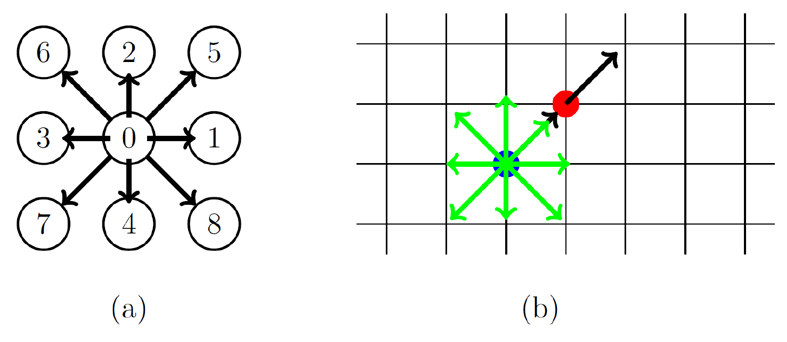
\includegraphics[width=9cm]{d2q9_scheme.png}
\end{figure}




% The equation arises not by analyzing the individual positions and momenta of each particle in the fluid but rather by considering a probability distribution for the position and momentum of a typical particle—that is, the probability that the particle occupies a given very small region of space (mathematically the volume element {\displaystyle \mathrm {d} ^{3}{\bf {r}}}{\displaystyle \mathrm {d} ^{3}{\bf {r}}}) centered at the position {\displaystyle {\bf {r}}}{\displaystyle {\bf {r}}}, and has momentum nearly equal to a given momentum vector {\displaystyle {\bf {p}}}{\displaystyle {\bf {p}}} (thus occupying a very small region of momentum space {\displaystyle \mathrm {d} ^{3}{\bf {p}}}{\displaystyle \mathrm {d} ^{3}{\bf {p}}}), at an instant of time.

The



.



\bibliographystyle{unsrt}
\bibliography{biblio}
% \bibliography{"/home/joe/repos/pylbm/milestones/final/biblio.bib"}

\end{document}
